\documentclass{beamer}
%\documentclass[handout]{beamer}

% This file is a solution template for:
% PHYS3202 Lectures
\mode<presentation>
{
  \usetheme{Madrid}
  \setbeamercovered{invisible}
\setbeamertemplate{footline}[frame number]{}
\setbeamertemplate{navigation symbols}{}
\setbeamertemplate{footline}{}
}
\usepackage[english]{babel}
\usepackage[latin1]{inputenc}
%\usepackage{times}
\usepackage[T1]{fontenc}

\renewcommand\familydefault{\sfdefault}

\usefonttheme[onlymath]{serif}


\usepackage[cm]{sfmath}

\newcommand{\td}[1]{\frac{D #1}{D t}}
\newcommand{\nd}[2]{\frac{d #1}{d #2}}
\newcommand{\ns}[2]{\frac{d^2 #1}{d #2^2}}
\newcommand{\sd}[2]{\frac{D #1}{D #2}}
\newcommand{\pd}[2]{\frac{\partial #1}{\partial #2}}
\newcommand{\ps}[2]{\frac{\partial^2 #1}{{\partial #2}^2}}
\newcommand{\pt}[2]{\frac{\partial^3 #1}{{\partial #2}^3}}
\newcommand{\pst}[3]{\frac{\partial^2 #1}{\partial #2 \partial #3}}
\newcommand{\ptt}[3]{\frac{\partial^3 #1}{{\partial #2}^2 \partial #3}}
\newcommand{\vc}[1]{\mathbf{#1}}
\newcommand{\mtx}[1]{\vc{\mathsf{#1}}}

%\sffamily



%\title[The Beta-Plane Approximation]{The Beta-Plane Approximation}

\title[Planetary Rossby Waves]{Planetary Rossby Waves}



%\[ \boxed{\frac{D}{Dt} \left( \frac{f + \zeta}{h}\right) = 0 }\]
%
%\[\frac{f + \zeta}{h} = q = {\textrm{constant along stream paths}}\] 


\author{$\quad\quad\quad\quad\quad\quad\quad\quad\quad\quad\quad\quad\quad\quad$Kial~Stewart}

\institute{
  $\quad\quad\quad\quad\quad\quad\quad\quad\quad\quad\quad\quad\quad\quad\quad\quad\quad\quad$Research School of Earth Sciences\\
  $\quad\quad\quad\quad\quad\quad\quad\quad\quad\quad\quad\quad\quad\quad\quad\quad\quad\quad$e: kial.stewart@anu.edu.au\\
  }

\date{$\quad\quad\quad\quad\quad\quad\quad\quad\quad\quad\quad\quad\quad\quad$PHYS 3202}

%%%%%%%%%%%%%%%%%%%%%%%%%%%%%%%

\begin{document}

\begin{frame}
  \titlepage
\end{frame} 

%%%%%%%%%%%%%%%%%%%%%%%%%%%%%%%



\frame{
  \frametitle{Planetary Rossby Waves}

   \begin{columns}
   \column{0.55\textwidth}

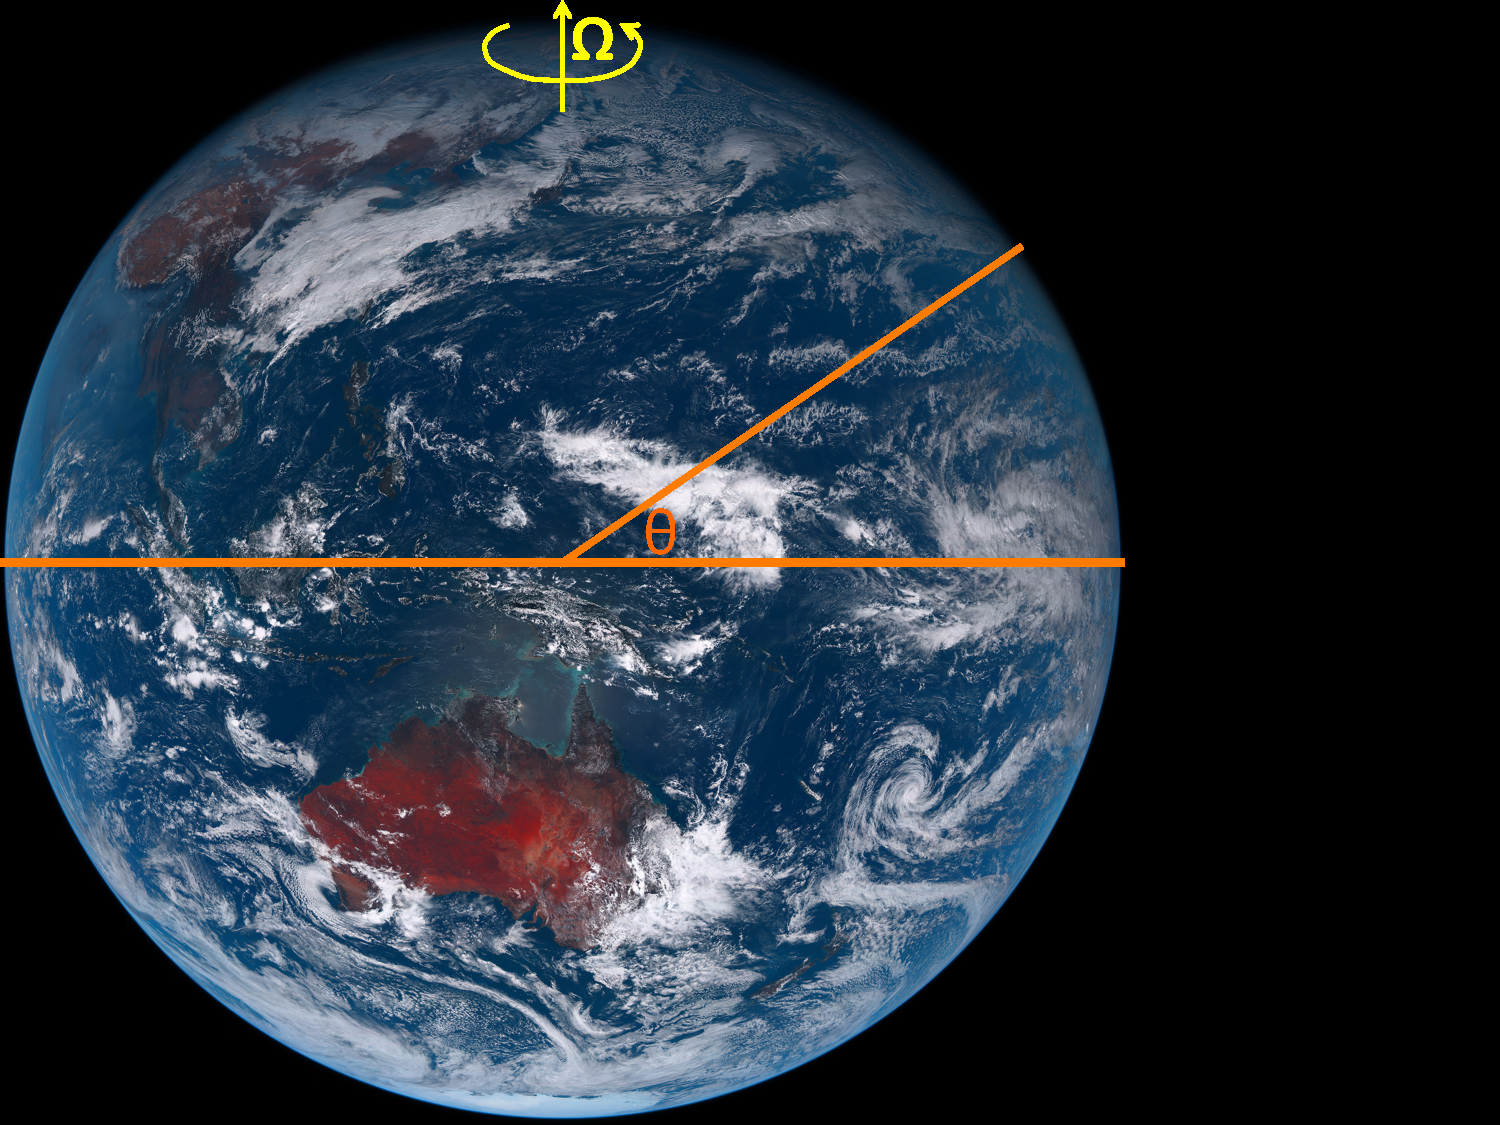
\includegraphics[width=1.0\hsize]{coriolis_04.pdf}


 \column{0.45\textwidth}
 
\center $f=2\Omega\textrm{sin}\Theta$
 
 \vskip1.0cm
 
 The Beta-Plane Approximation:

$ f = f_{0} + \beta{y} $,\\

 \vskip0.5cm

 
where $f_{0} = 2\Omega\textrm{sin}\Theta_{0}$ and $\beta \approx \frac{\partial{f}}{\partial{y}}$.

 
 
   \end{columns}


}

%
%
%\[ \boxed{\frac{\partial{\eta}}{\partial{t}} - R^{2} \frac{\partial}{\partial{t}}\nabla^{2}\eta - R^{2}\beta\frac{\partial\eta}{\partial{x}} = 0} \hskip3cm (9)\]
%


%
%\frame{
%  \frametitle{Rossby Waves - motivation}
%\center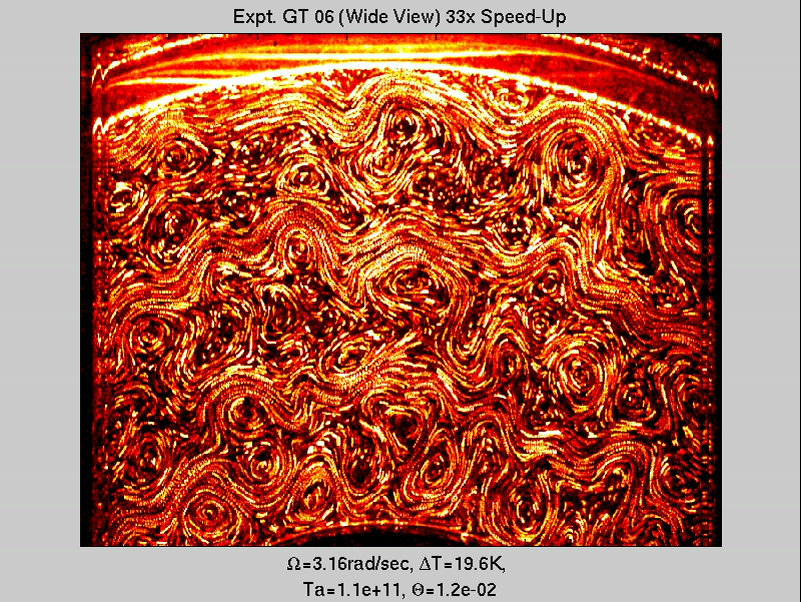
\includegraphics[width=0.7\hsize]{shot0002.png}
%
%\center A rotating tank with radial sloping bottom ($\partial{H}/\partial{r}\neq0$). Flow is forced by a radial temperature difference.
%
%}




%
%
%\frame{
%  \frametitle{Conserving Potential Vorticity}
%
%\[ \boxed{\frac{D}{Dt} \left( \frac{f + \zeta}{h}\right) = 0 }\]
%
%\[\frac{f + \zeta}{h} = q = {\textrm{constant along stream paths}}\] 
%
% \begin{alertblock}{Potential Vorticity a conserved quantity}
% Provides a means for predicting the evolution of flow
% \end{alertblock}
%
%\vskip1.0cm
%\quad\quad\quad\quad\quad\quad What happens when $f$ or $h$ change?
%
%}
%%
%%
%%
%%
%%%%%%%%%%%%%%%%%%%%%%%%%%%%%%%%%
%
%\frame{
%  \frametitle{Beta-plane approximation: variation of $f$ with latitude}
%
%\begin{itemize}
%
%\item Coriolis parameter $f=2\Omega{\textrm{sin}}\theta$ is not globally uniform.
%
%\pause
%
%\item This needs to be accounted for in flows with large latitudinal extent.
%
%\pause
%
%\item A useful approximation is to take $\theta = \theta_{0} + y/R_{E}$, where $R_{E}$ is radius of Earth, so
%
%\pause
%
%\[ f = 2\Omega\left( {\textrm{sin}}\theta_{0} + \frac{y}{R_{E}}{\textrm{cos}}\theta_{0} + \left(\frac{y}{R_{E}}\right)^{2}{\textrm{sin}}^{2}\theta_{0} + ... \right) \]
%
%\pause
%
%Retain the first two terms,
%
%\[ f = f_{0} + \beta{y} \]
%
%where $f_{0} = 2\Omega{\textrm{sin}}\theta_{0}$, and $\beta=2\frac{\Omega}{R_{E}}{\textrm{cos}}\theta_{0} \approx \partial{f}/\partial{y}$
%
%\pause
%
%\item This is the ``Beta-plane approximation''
%
%\end{itemize}
%}
%
%%%%%%%%%%%%%%%%%%%%%%%%%%%%%%%%
%
%\frame{
%  \frametitle{Planetary Rossby Waves}
%
%Begin with the assumptions for conserving potential vorticity: inviscid, thin, `rapid' rotation.
%
%\[ \boxed{\frac{D}{Dt} \left( \frac{f + \zeta}{h}\right) = 0 }\]
%
%\pause
%
%The equations describing horizontal motions are:
%
% \[\pd{u}{t} + {u \pd{u}{x} +  v \pd{u}{y} + w\pd{u}{z}} - fv = -\frac{1}{\rho}\pd{p}{x} \hskip1cm (1)\]
% \[\pd{v}{t} + { u \pd{v}{x} +  v \pd{v}{y} + w\pd{v}{z}} + fu = -\frac{1}{\rho}\pd{p}{y} \hskip1cm (2)\]
%  \[ \pd{u}{x} +  \pd{v}{y} + \pd{w}{z} = 0  \hskip3cm (3) \]
%  
%.
%
%.
%}
%
%
%%%%%%%%%%%%%%%%%%%%%%%%%%%%%%%%
%
%\frame{
%  \frametitle{Planetary Rossby Waves}
%
%Begin with the assumptions for conserving potential vorticity: inviscid, thin, `rapid' rotation.
%
%\[ \boxed{\frac{D}{Dt} \left( \frac{f + \zeta}{h}\right) = 0 }\]
%
%%\pause
%
%The equations describing horizontal motions are:
%
% \[\pd{u}{t} + {\color{red}u \pd{u}{x} +  v \pd{u}{y} + w\pd{u}{z}} - fv = -\frac{1}{\rho}\pd{p}{x} \hskip1cm (1)\]
% \[\pd{v}{t} + {\color{red} u \pd{v}{x} +  v \pd{v}{y} + w\pd{v}{z}} + fu = -\frac{1}{\rho}\pd{p}{y} \hskip1cm (2)\]
%  \[ \pd{u}{x} +  \pd{v}{y} + \pd{w}{z} = 0  \hskip3cm (3) \]
%  
%Consider fluctuations with no mean flow (e.g., waves) and small velocities (small $Ro$), so {\color{red}neglect nonlinear advection} terms.
%}
%
%
%%%%%%%%%%%%%%%%%%%%%%%%%%%%%%%%
%
%\frame{
%  \frametitle{Planetary Rossby Waves}
%
% \[\pd{u}{t} - fv = -\frac{1}{\rho}\pd{p}{x} \hskip1cm (1)\]
% \[\pd{v}{t} + fu = -\frac{1}{\rho}\pd{p}{y} \hskip1cm (2)\]
%%  \[ \pd{u}{x} +  \pd{v}{y} + \pd{w}{z} = 0  \hskip3cm (3) \]
% \pause 
%Substitute for $f = f_{0} + \beta{y}$,
%
% \[\pd{u}{t} - \left(f_{0} + \beta{y}\right)v = -\frac{1}{\rho}\pd{p}{x} \hskip1cm (1)\]
% \[\pd{v}{t} + \left(f_{0} + \beta{y}\right)u = -\frac{1}{\rho}\pd{p}{y} \hskip1cm (2)\]
%%  \[ \pd{u}{x} +  \pd{v}{y} + \pd{w}{z} = 0  \hskip3cm (3) \]
%
%
%}
%
%
%%%%%%%%%%%%%%%%%%%%%%%%%%%%%%%%
%
%\frame{
%  \frametitle{Planetary Rossby Waves}
%
% \[\pd{u}{t} - \left(f_{0} + \beta{y}\right)v = -\frac{1}{\rho}\pd{p}{x} \hskip1cm (1)\]
% \[\pd{v}{t} + \left(f_{0} + \beta{y}\right)u = -\frac{1}{\rho}\pd{p}{y} \hskip1cm (2)\]
%%  \[ \pd{u}{x} +  \pd{v}{y} + \pd{w}{z} = 0  \hskip3cm (3) \]
%% \pause 
%and replace pressure gradients with surface height anomalies $\eta$,
%
%that is, $\frac{1}{\rho} \frac{\partial{p}}{\partial{x}} = g \frac{\partial{\eta}}{\partial{x}}$ (hydrostatic),
%
% \[\pd{u}{t} - \left(f_{0} + \beta{y}\right)v = -g\pd{\eta}{x} \hskip1cm (1)\]
% \[\pd{v}{t} + \left(f_{0} + \beta{y}\right)u = -g\pd{\eta}{y} \hskip1cm (2)\]
%%  \[ \pd{u}{x} +  \pd{v}{y} + \pd{w}{z} = 0  \hskip3cm (3) \]
%
%
%}
%
%
%%%%%%%%%%%%%%%%%%%%%%%%%%%%%%%%
%
%
%\frame{
%  \frametitle{Planetary Rossby Waves}
%
% \[ {\color{blue}\pd{u}{t}} - \left(f_{0} + {\color{blue}\beta{y}}\right)v = -g\pd{\eta}{x} \hskip1cm (1)\]
% \[ {\color{blue}\pd{v}{t}} + \left(f_{0} + {\color{blue}\beta{y}}\right)u = -g\pd{\eta}{y} \hskip1cm (2)\]
%
%Recall that the flow is predominantly geostrophic, so the {\color{blue}time-dependent} and {\color{blue}beta} terms are small compared to geostrophy.
%
%\pause
%
%\begin{itemize}
%
%\item As the geostrophic terms dominate, use these to express the velocities as,
%\[ u \approx -\frac{g}{f_{0}}\frac{\partial{\eta}}{\partial{y}}, \quad  v \approx \frac{g}{f_{0}}\frac{\partial{\eta}}{\partial{x}} \]
%
%\pause
%
%and substitute back into (1,2) for the {\color{blue}small terms}:
%
% \[ {\color{blue}-\frac{g}{f_{0}}\frac{\partial^{2}{\eta}}{\partial{y}\partial{t}}} - f_{0}v {\color{blue}-\beta{y}\frac{g}{f_{0}}\frac{\partial{\eta}}{\partial{x}}} = -g\pd{\eta}{x} \hskip1cm (4)\]
% \[ {\color{blue}+\frac{g}{f_{0}}\frac{\partial^{2}{\eta}}{\partial{x}\partial{t}}} + f_{0}u {\color{blue}-\beta{y}\frac{g}{f_{0}}\frac{\partial{\eta}}{\partial{y}}} = -g\pd{\eta}{y} \hskip1cm (5)\]
%
%\end{itemize}
%
%}
%
%
%%%%%%%%%%%%%%%%%%%%%%%%%%%%%%%%
%
%\frame{
%  \frametitle{Planetary Rossby Waves}
%
% \[ {\color{blue}-\frac{g}{f_{0}}\frac{\partial^{2}{\eta}}{\partial{y}\partial{t}}} - f_{0}v {\color{blue}-\beta{y}\frac{g}{f_{0}}\frac{\partial{\eta}}{\partial{x}}} = -g\pd{\eta}{x} \hskip1cm (4)\]
% \[ {\color{blue}+\frac{g}{f_{0}}\frac{\partial^{2}{\eta}}{\partial{x}\partial{t}}} + f_{0}u {\color{blue}-\beta{y}\frac{g}{f_{0}}\frac{\partial{\eta}}{\partial{y}}} = -g\pd{\eta}{y} \hskip1cm (5)\]
%
%Rearrange (4,5) for $v$ and $u$:
%
%\pause
%
% \[ v =  +\frac{g}{f_{0}}\pd{\eta}{x} {\color{blue}-\frac{g}{f_{0}^{2}}\frac{\partial^{2}{\eta}}{\partial{y}\partial{t}}} {\color{blue}-\beta{y}\frac{g}{f_{0}^{2}}\frac{\partial{\eta}}{\partial{x}}}  \hskip1cm (6)\]
% \[ u =  -\frac{g}{f_{0}}\pd{\eta}{y} {\color{blue}-\frac{g}{f_{0}^{2}}\frac{\partial^{2}{\eta}}{\partial{x}\partial{t}}} {\color{blue}+\beta{y}\frac{g}{f_{0}^{2}}\frac{\partial{\eta}}{\partial{y}}}  \hskip1cm (7)\]
%
%\pause
%
%The {\color{blue} blue} terms are {\color{blue} ageostrophic}. These describe the behaviour of the wave perturbations superimposed on the geostrophic flow.
%
%}
%
%%%%%%%%%%%%%%%%%%%%%%%%%%%%%%%%
%
%\frame{
%  \frametitle{Planetary Rossby Waves}
%
%Recall (3), the continuity equation,
%  \[ \pd{u}{x} +  \pd{v}{y} + \pd{w}{z} = 0  \hskip3cm (3) \]
%\pause
%This can be integrated over a layer depth $H$,
%
%  \[ \int_{0}^{H}\left(\pd{u}{x} +  \pd{v}{y} + \pd{w}{z}\right)dz = H\left( \pd{u}{x} +  \pd{v}{y}\right) + w(H) - w(0) = 0 \]
%  \[ \frac{\partial{\eta}}{\partial{t}} + H\left( \pd{u}{x} +  \pd{v}{y}\right) = 0 \hskip3cm (8)\]
%
%\pause
%
%Substitute $u,v$ from (6,7) into (8):
%
%}
%
%%%%%%%%%%%%%%%%%%%%%%%%%%%%%%%%
%
%\frame{
%  \frametitle{Planetary Rossby Waves}
%Substitute $u,v$ from (6,7) into (8):
% \[ v =  +\frac{g}{f_{0}}\pd{\eta}{x} {\color{blue}-\frac{g}{f_{0}^{2}}\frac{\partial^{2}{\eta}}{\partial{y}\partial{t}}} {\color{blue}-\beta{y}\frac{g}{f_{0}^{2}}\frac{\partial{\eta}}{\partial{x}}}, \quad  u =  -\frac{g}{f_{0}}\pd{\eta}{y} {\color{blue}-\frac{g}{f_{0}^{2}}\frac{\partial^{2}{\eta}}{\partial{x}\partial{t}}} {\color{blue}+\beta{y}\frac{g}{f_{0}^{2}}\frac{\partial{\eta}}{\partial{y}}} \quad (6,7)\]
% \[ \frac{\partial{\eta}}{\partial{t}} + H\left( \pd{u}{x} +  \pd{v}{y}\right) = 0 \hskip3cm (8) \]
%\pause
% \[ \frac{\partial{\eta}}{\partial{t}} + \frac{gH}{f_{0}^{2}}\left( \pd{}{x}\left[-{f_{0}}\pd{\eta}{y} {\color{blue}-\frac{\partial^{2}{\eta}}{\partial{x}\partial{t}}} {\color{blue}+\beta{y}\frac{\partial{\eta}}{\partial{y}}} \right] +  \pd{}{y}\left[ +{f_{0}}\pd{\eta}{x} {\color{blue}-\frac{\partial^{2}{\eta}}{\partial{y}\partial{t}}} {\color{blue}-\beta{y}\frac{\partial{\eta}}{\partial{x}}}\right]\right) = 0 \]
%\pause
% \[ \frac{\partial{\eta}}{\partial{t}} + \frac{gH}{f_{0}^{2}}\left( {\color{blue}- \frac{\partial^{3}\eta}{\partial{x}^{2}\partial{t}}  - \frac{\partial^{3}\eta}{\partial{y}^{2}\partial{t}}  - \beta\frac{\partial\eta}{\partial{x}} }\right) = 0\] 
%\pause
% \[ \frac{\partial{\eta}}{\partial{t}} + \frac{gH}{f_{0}^{2}}\left( {\color{blue}- \frac{\partial}{\partial{t}}\left[ \frac{\partial^{2}\eta}{\partial{x}^{2}}  + \frac{\partial^{2}\eta}{\partial{y}^{2}}\right]  - \beta\frac{\partial\eta}{\partial{x}} }\right) = 0\] 
%% \[ \frac{\partial{\eta}}{\partial{t}} + \frac{gH}{f_{0}^{2}}\left(-{f_{0}}\frac{\partial^{2}\eta}{\partial{x}\partial{y}} - \frac{\partial^{3}\eta}{\partial{x}^{2}\partial{t}} +\beta{y}\frac{\partial^{2}\eta}{\partial{x}\partial{y}} + \frac{\partial^{2}\eta}{\partial{x}\partial{y}} - \frac{\partial^{3}\eta}{\partial{y}^{2}\partial{t}} - \beta{y}\frac{\partial^{2}\eta}{\partial{x}\partial{y}}  - \beta\frac{\partial\eta}{\partial{x}} \right) = 0\] 
%}
%
%%%%%%%%%%%%%%%%%%%%%%%%%%%%%%%%
%
%\frame{
%  \frametitle{Planetary Rossby Waves}
% \[ \frac{\partial{\eta}}{\partial{t}} + \frac{gH}{f_{0}^{2}}\left( {\color{blue}- \frac{\partial}{\partial{t}}\left[ \frac{\partial^{2}\eta}{\partial{x}^{2}}  + \frac{\partial^{2}\eta}{\partial{y}^{2}}\right]  - \beta\frac{\partial\eta}{\partial{x}} }\right) = 0\] 
%Substitute for $\nabla^{2}\eta=\frac{\partial^{2}\eta}{\partial{x}^{2}}+\frac{\partial^{2}\eta}{\partial{y}^{2}}$ and define $R = \frac{\sqrt{gH}}{f_{0}}$ as the Rossby radius:
% \[ \boxed{\frac{\partial{\eta}}{\partial{t}} - R^{2} \frac{\partial}{\partial{t}}\nabla^{2}\eta - R^{2}\beta\frac{\partial\eta}{\partial{x}} = 0} \hskip3cm (9)\] 
%
%\quad\quad This is the Rossby wave equation.
%
%\pause
%The coefficients of (9) are constant, and we have assumed the perturbation is a wave, so we prescribe form $\eta = \eta_{0}{\textrm{cos}}\left(kx - my - \omega{t}\right)$.
%\pause
%This allows us to rewrite (9) in terms of $\omega$ as a dispersion relation for Rossby waves:
%
%\[ \boxed{\omega = -\beta{R^{2}}\frac{k}{1+R^{2}\left( k^{2} + m^{2} \right)}} \]
%
%% \[ \frac{\partial{\eta}}{\partial{t}} + \frac{gH}{f_{0}^{2}}\left(-{f_{0}}\frac{\partial^{2}\eta}{\partial{x}\partial{y}} - \frac{\partial^{3}\eta}{\partial{x}^{2}\partial{t}} +\beta{y}\frac{\partial^{2}\eta}{\partial{x}\partial{y}} + \frac{\partial^{2}\eta}{\partial{x}\partial{y}} - \frac{\partial^{3}\eta}{\partial{y}^{2}\partial{t}} - \beta{y}\frac{\partial^{2}\eta}{\partial{x}\partial{y}}  - \beta\frac{\partial\eta}{\partial{x}} \right) = 0\] 
%}
%
%
%%%%%%%%%%%%%%%%%%%%%%%%%%%%%%%%
%
%\frame{
%  \frametitle{Planetary Rossby Waves - frequencies}
%
%Dispersion relation for planetary Rossby waves (recall $R = \sqrt{gH}/f_{0}$):
%\[ \boxed{\omega = -\beta{R^{2}}\frac{k}{1+R^{2}\left( k^{2} + m^{2} \right)}} \]
%\pause
%\begin{itemize}
%\item For $\beta = 0$ $\rightarrow$ $\omega=0$: steady, geostrophic flow at constant $f$ (no waves)
%\pause
%\item We have assumed $Ro<<1$, so solution only valid for $\omega<<f_{0}$
%\pause
%\item Consider $k,m\sim{1/L}$ $\rightarrow$ $\omega \sim \beta{R^2}L/(L^2 + R^2)$:
%\pause
%\item so for short waves $L<R$: $\omega\sim\beta{L}$
%\pause
%\item for long waves $L>R$: $\omega\sim\beta{R^2}/{L}$ \pause $< \beta{L}$
%\pause
%\item for $L=R$: $\omega$ is maximum at $|\omega_{max}| = \beta{R}/2$
%\end{itemize}
%
%}
%
%%%%%%%%%%%%%%%%%%%%%%%%%%%%%%%%
%
%\frame{
%  \frametitle{Planetary Rossby Waves - propagation}
%
%Dispersion relation for planetary Rossby waves (recall $R = \sqrt{gH}/f_{0}$):
%\[ \boxed{\omega = -\beta{R^{2}}\frac{k}{1+R^{2}\left( k^{2} + m^{2} \right)}} \]
%\pause
%\begin{itemize}
%\item ZONAL phase speed always negative $\rightarrow$ westward propagation
%\[ c_{x} = \frac{\omega}{k} = - \beta{R^{2}}\frac{1}{1+R^{2}\left( k^{2} + m^{2} \right)}\]
%\pause
%\item MERIDIONAL phase speed either sign
%\[ c_{y} = \frac{\omega}{m} = - \beta{R^{2}}\frac{k/m}{1+R^{2}\left( k^{2} + m^{2} \right)}\]
%\pause
%\item Very long waves ($1/k, 1/m, L >> R$):\\
% propagate westward at $c = -\beta{R^{2}}$, maximum speed allowed
%\end{itemize}
%
%}
%
%
%%%%%%%%%%%%%%%%%%%%%%%%%%%%%%%%
%
%\frame{
%  \frametitle{Topographic Rossby Waves}
%
%%Planetary Rossby waves travel on the north-south gradient of $f$. What about gradients of $h$?
%Recall the conservation of Potential Vorticity (PV)
%\[ \boxed{\frac{D}{Dt}\left(\frac{f+\zeta}{h}\right)=0}\]
%
%where $q=(f+\zeta)/h$ is the PV.
%
%\pause
%\begin{itemize}
%\item Allow for a ``beta-plane'', so PV becomes $q=(f_{0} + \beta{y}+\zeta)/h$ 
%\pause
%\item For sloping bottom, allow fluid depth to be $h = h_{0} + \alpha{y} + \eta(x,y,t)$
%\pause
%\item Allow $\alpha{y}$ to replace $\beta{y}$, so PV becomes $q=(f_{0} - \alpha{y}+\zeta)/(h_{0} + \eta)$
%\pause
%\item Repeat the derivation for planetary waves but with $\alpha{y}$ in place of $\beta{y}$ and variable depth $h$
%\pause
%
%\[ \boxed{ \omega_{T} = \frac{\alpha{g}}{f_{0}}\frac{k}{1+R^{2}\left(k^{2} + m^{2}\right)} } \]
%
%\end{itemize}
%
%\begin{itemize}
%\item Long waves have maximum speed $c = \alpha{g}/f_{0}$ along isobaths.
%\pause
%\item Maximum frequency of $|\omega_{T,max} | = | \alpha{g}/2f_{0}R| = | (\alpha/2)\sqrt{(g/H)}|$
%\end{itemize}
%
%}
%
%%%%%%%%%%%%%%%%%%%%%%%%%%%%%%%%
%
%  
%  
%\section{Physical explanation of Rossby waves}
%
%
%\frame{
%  \frametitle{Physical explanation of Planetary Rossby waves}
% \[\boxed{\sd{}{t}\left(\frac{f+\zeta}{h}\right)=0}  \]
%\includegraphics[width=1.0\hsize]{prossby1.pdf}
%
%}
%
%
%\frame{
%  \frametitle{Physical explanation of Planetary Rossby waves}
% \[\boxed{\sd{}{t}\left(\frac{f+\zeta}{h}\right)=0}  \]
%\includegraphics[width=1.0\hsize]{prossby2.pdf}
%
%}
%
%
%\frame{
%  \frametitle{Physical explanation of Planetary Rossby waves}
% \[\boxed{\sd{}{t}\left(\frac{f+\zeta}{h}\right)=0}  \]
%\includegraphics[width=1.0\hsize]{prossby3.pdf}
%
%}
%
%
%\frame{
%  \frametitle{Physical explanation of Planetary Rossby waves}
% \[\boxed{\sd{}{t}\left(\frac{f+\zeta}{h}\right)=0}  \]
%\includegraphics[width=1.0\hsize]{prossby4.pdf}
%
%}
%
%
%\frame{
%  \frametitle{Physical explanation of Planetary Rossby waves}
% \[\boxed{\sd{}{t}\left(\frac{f+\zeta}{h}\right)=0}  \]
%\includegraphics[width=1.0\hsize]{prossby5.pdf}
%
%}
%
%
%\frame{
%  \frametitle{Physical explanation of Topographic Rossby waves}
% \[\boxed{\sd{}{t}\left(\frac{f+\zeta}{h}\right)=0}  \]
%\includegraphics[width=1.0\hsize]{trossby1.pdf}
%
%}
%
%
%\frame{
%  \frametitle{Physical explanation of Topographic Rossby waves}
% \[\boxed{\sd{}{t}\left(\frac{f+\zeta}{h}\right)=0}  \]
%\includegraphics[width=1.0\hsize]{trossby2.pdf}
%
%}
%
%
%
%
%
%\frame{
%  \frametitle{Physical explanation of Rossby waves}
%  We must conserve PV.
%  
%    \begin{columns}
%    \column{0.4\textwidth}
%\includegraphics[width=1.0\hsize]{prossby5.pdf}
%
%\includegraphics[width=1.0\hsize]{trossby1.pdf}
%
%\includegraphics[width=1.0\hsize]{trossby2.pdf}
%
%  \column{0.6\textwidth}
%\pause
%  \begin{itemize}
%  \item {\color{blue} \textit{Planetary Rossby waves}:} $f$ variations require changes in relative vorticity $\zeta$ to conserve PV.
%  \pause
%   \item {\color{purple} \textit{Topographic Rossby waves}:} depth variations require changes in $\zeta$ to conserve PV.
%   \pause
%  \item These changes in $\zeta$ lead to movement of crests and troughs along {\color{blue}lines of latitude} or {\color{purple}isobaths}. 
%  \end{itemize}
%  \pause
%     \begin{exampleblock}{traveling wave solutions}
%phase propagates with smaller $q_0 = f/h$ on the left ({\color{blue}westward in both hemispheres}); {\color{purple}deeper on left in Nth (right in Sth) hemispheres}.
%   \end{exampleblock}
%  
%      \end{columns}
%
%  }
%  
%%  
%%  %%%%%%%%%%%%%%%%%%%%%%
%%  
%%  \frame{
%%  \frametitle{Question: Rossby waves in lee of topography}
%%\center{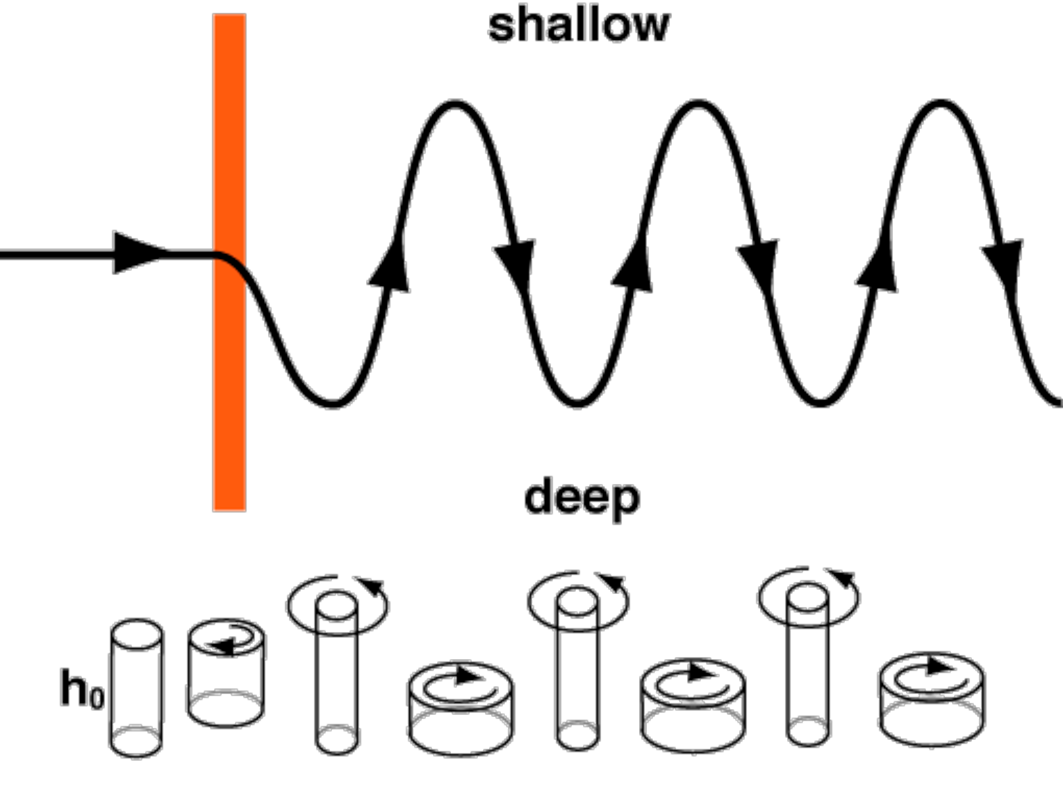
\includegraphics[width=0.65\hsize]{rossbyleewavesketch_cropped.pdf}}
%%
%%Imagine eastward flow encountering a topographic ridge.
%%
%%Sketch the evolution of the flow as it crosses the ridge and downstream of the ridge.
%%
%%
%%%Rossby waves in eastward flow (Northern hemisphere), generated by
%%%compression/stretching of vortex columns over the topography.   
%%%North-South gradient of $f$ supports Rossby waves downstream.
%%
%%}
%%
%
%
%
%


\end{document}







































